\section{Tendencias}

% \subsection{Diplomas Digitales Argentina }
% Las certificaciones digitales del ámbito académico aumentaron su uso en el último tiempo; un ejemplo de ello es  
% la Universidad de Buenos Aires (UBA), que expide sus títulos por un sistema online que acorta el tiempo 
% a dos meses generando un documento digital de  formato pdf encriptado. En el sitio web describen que los diplomas digitales 
% corresponden a carreras  de grado, acreditaciones parciales de una carrera de grado, carreras técnicas de nivel universitario, de 
% complementación curricular de una carrera de grado y  de posgrado también certificados de reválida expedidos 
% por la Universidad y certificados analíticos finales \cite[]{facultad_de_farmacia_y_bioquimica_universidad_de_buenos_aires_diploma_2020}.

% Asi mismo el Rectorado de la UBA, dispuso mediante la Resolución {RESCS}-2020-271-{E}-{UBA}-{REC}\cite[]{universidad_de_buenos_aires_resolucion_2020}  
% Define que "Los diplomas serán firmados digitalmente con dispositivo
% criptográfico por el o la Rectora y el o la Secretaria de Asuntos Académicos de esta
% Universidad; la/s o lo/s Decano/s y el o la Secretaria/s Académica/s de la/s
% Facultad/es. El Director o Directora General de la Dirección General de Títulos y
% Planes certificará con su firma digital toda la información que deba constar de
% acuerdo con el tipo de diploma expedido.
% Sin perjuicio de su firma digital, en el anverso de los diplomas se reproducirán las
% firmas ológrafas y se consignará los nombres, apellidos y cargo de las autoridades
% indicadas en el párrafo precedente. En el reverso, se reproducirá la firma ológrafa
% del Director o Directora General de la Dirección General de Títulos y Planes."\cite[]{universidad_de_buenos_aires_anexo1_2020}

% De esta forma, se observa que la universidad utiliza el método de firma digital para asegurar la integridad de los documentos digitales.
% En la resolución mencionada se muestran los modelos de los certificados y son considerados documentos digitales en sí. La Figura \ref{img:modelo1-certificado}  representa el 
% Modelo 1, este documento corresponde a una carrera técnica de nivel universitario o carrera de grado completa 
% dependiente de un Facultad  \cite[]{universidad_de_buenos_aires_anexo2_2020}. 

% \begin{figure}[hbt!]
%     \centering
%     {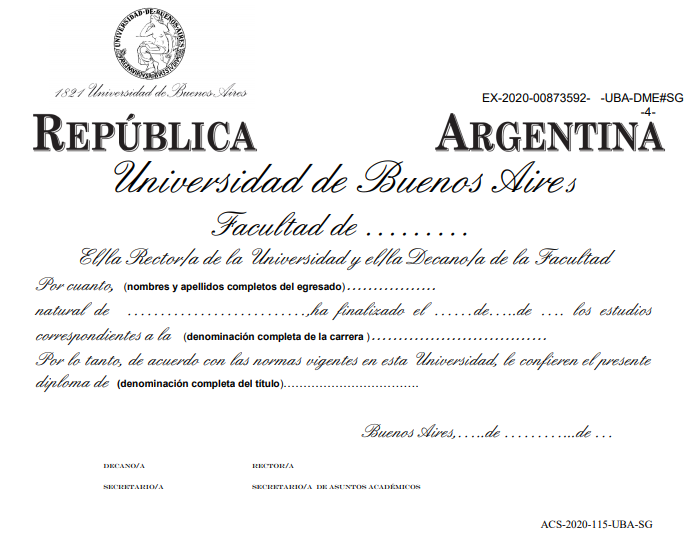
\includegraphics[scale=0.7]{modelo1-certificado.png}}
%     \caption{Modelo 1 de Certificado} 
%     \label{img:modelo1-certificado}
% \end{figure}


% Los certificados digitales también son utilizados en  la Universidad Nacional De La Plata (UNLP) 
%  ya que la entrega de los títulos es completamente online y los primeros en recibirlos
% fueron estudiantes de la Licenciatura en Sistemas. El proceso de emisión del  título  hasta que lo reciben los egresados de las 
% carreras ha mejorado significativamente, ya que  testimonios de esperar 
% meses los títulos ahora lo reciben en cuestiones de días \cite[]{unlp_certificado_2020}.


% En cuanto a las tendencias de la tecnología Blockchain, resaltan 
% la creación de proyectos relacionados al ámbito financiero, mientras que en otras áreas como identidad digital, votos, sectores académicos 
% se la utiliza pero siguen siendo más consultada y en cantidad el uso financiero como creación
% de monedas digitales y ecosistemas que permiten a las personas utilizarlos.\cite[]{preukschat_Blockchain_2018,drescher_Blockchain_2017}

% \subsection{Las Tecnologías Digitales }
 La Blockchain  cada día es utilizado por distintos sectores para respaldar 
documentos, asi también en casos de agricultura, y cada vez se muestran nuevos proyectos \cite[]{Blockchain_federal_argentina_trazabilidad_nodate}. 

Actualmente el mundo del  Blockchain está en crecimiento con los proyectos relacionados a los 
criptoactivos, la gran mayoría de los consumidores de esta tecnología lo usan para generar 
ganancias o ingresos con las distintas manera que  ofrecen los proyectos.
Existen sistemas web que públican las criptoactivos con mayor relevancia según el relevamiento que realizan ellos, 
dos de estos sistemas web son CoinMarketCap y CoinGecko.

% \begin{figure}[hbt!]
%     \centering
%     {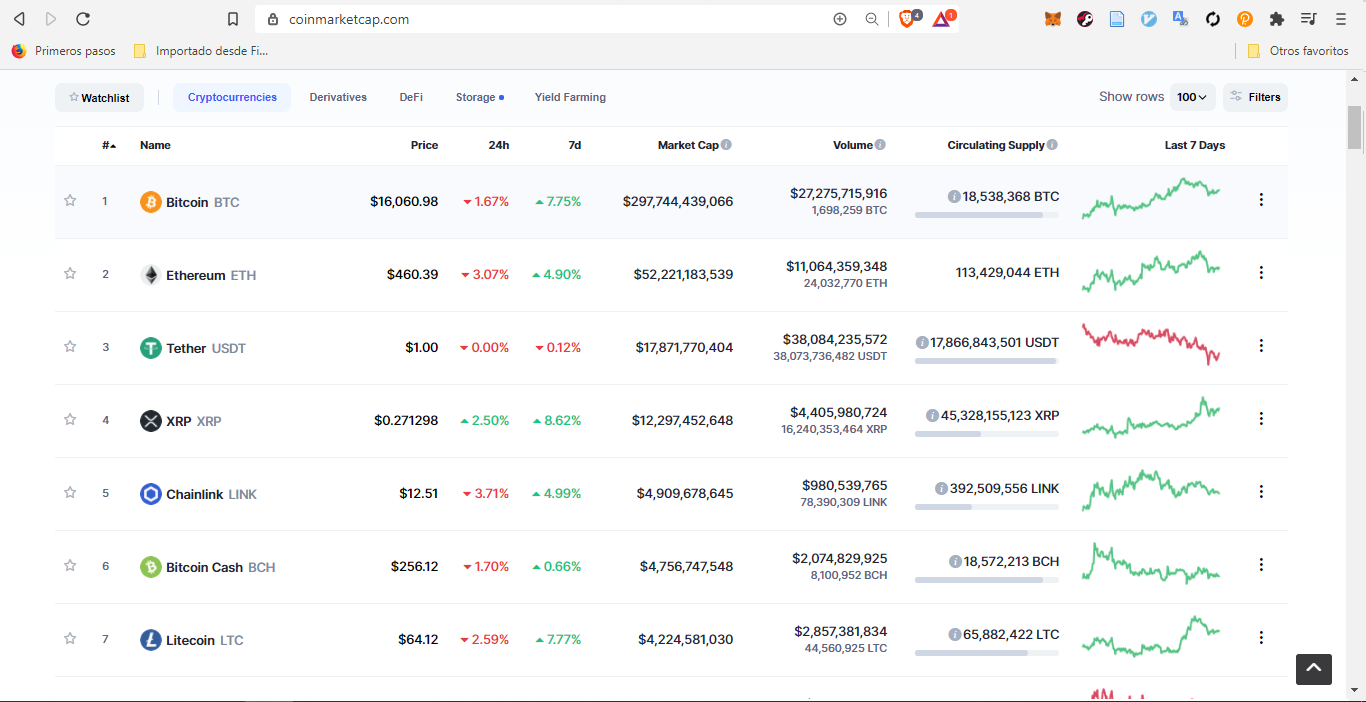
\includegraphics[scale=0.4]{coinmarketcap-valores.png}}
%     \caption{Captura de pantalla de la  página CoinMarketCap el 14/11/2020 a las 21:23 hs Argentina} 
%     \label{img:coinmarketcap-valores}
% \end{figure}

% \begin{figure}[hbt!]
%     \centering
%     {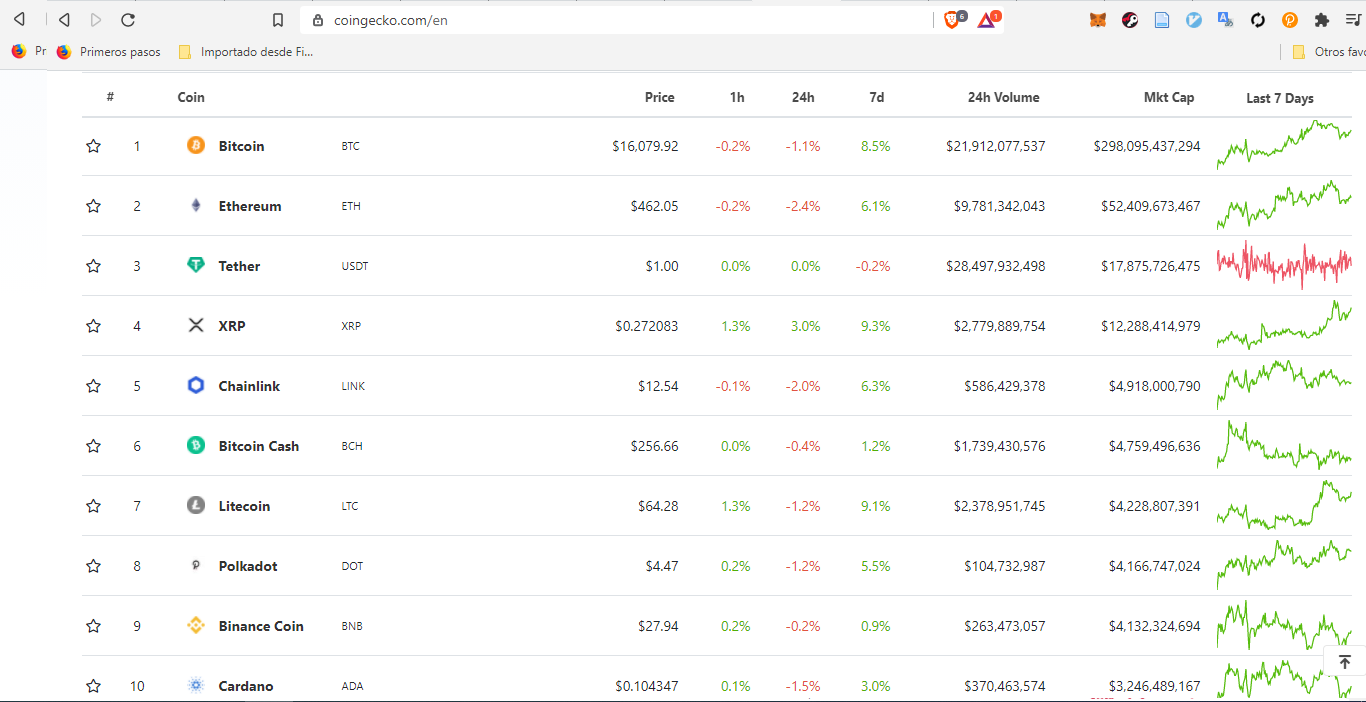
\includegraphics[scale=0.4]{coingecko-valores.png}}
%     \caption{Captura de pantalla de la  página CoinGecko el 14/11/2020 a las 21:23 hs Argentina} 
%     \label{img:coingecko-valores}
% \end{figure}

% En la  Figura \ref{img:coinmarketcap-valores} 
%  y 
% Figura \ref{img:coingecko-valores}     
% muestra una lista de los criptomonedas y los tokens con mayor capital de mercados.
Generalmente los  dos primeros puestos se están Bitcoin (BTC) y el Ether (ETH) que son criptomonedas nativa de su Blockchain. 
Asi como estas monedas digitales existen un sin numero de ellas y se crean constantemente, donde su valor reside en la oferta y demanda,
si no hay demanda por la obtención de un activo digital, no tiene valor \cite[]{joaquin_lopez_lerida_economiBlockchain_2016}.

Por otro lado el gobierno Argentino impulsa un proyecto de ley relacionadas a las criptomonedas y activos digitales,
el objetivo es crear un marco regulatorio integral, aplicable a las transacciones y operaciones civiles y 
comerciales de criptoactivos  y permitir
el crecimiento del ecosistema local  \cite[]{dagostino_exclusivo_nodate}.


El artículo \cite[]{dagostino_exclusivo_nodate} describe que la promulgación de esta ley permitirá:
\begin{enumerate}
    \item El Estado pueda determinar qué \glsplural{proyecto_cripto} autoriza y cuáles no en base criterios legales que hoy no existen.

    \item Las empresas tengan modelos de negocios que cumplan con ciertos criterios, como una  Blockchain pública o casos de uso.

    \item Se puedan representar tenencias de acciones, una propiedad, etcétera.

\end{enumerate}


La definición de un criptoactivo posibilitará que las capitales de riesgos internacionales 
que pretenden invertir tengan  seguridad jurídica y la certeza destinado los fondos \cite[]{dagostino_exclusivo_nodate}. 

% Esto no es nuevo, en países como EE.UU., China, Rusia se 
% encuentran operando con monedas digitales gubernamentales y expresan que será un punto de partida para crear nuevos servicios y obtener un liderazgo a nivel regional
% como global \cite[]{dagostino_exclusivo_nodate}.

La Cámara de Diputados de la Provincia de Misiones de Argentina aprobó el proyecto denominado como 
Programa Misionero de Innovación Financiera con Tecnología Blockchain y Criptomoneda. A partir del proyecto
la Provincia podra emitir su propia Criptomoneda y almacenar datos de la administración pública en la Blockchain.
Los objetivos principales son emitir una propia StableCoin (Moneda Estable) que usara la Provincia como herramienta de financiación entre el sector público
y privado, otro uso es la gestión de datos para la administración pública y por último la emisión de certificados verdes con el uso de la tecnología 
usarlo para validar titulo o certificados. \cite[]{clementin_provincia_2021}


